%%%%%%%%%%%%%%%%%%%%%%%%%%%%%%%%%%%%%%%%%%%%%%%%%%%%%%%%%%%%%%%%%%%%%%%%%%%%%%%%%
% Template: Article
%
% Por: Abrantes Araújo Silva Filho
%      abrantesasf@gmail.com
%
% Citação: Se você gostou deste template, por favor ajude a divulgá-lo mantendo
%          o link para meu repositório GitHub em:
%          https://github.com/abrantesasf/LaTeX
%%%%%%%%%%%%%%%%%%%%%%%%%%%%%%%%%%%%%%%%%%%%%%%%%%%%%%%%%%%%%%%%%%%%%%%%%%%%%%%%%





%%%%%%%%%%%%%%%%%%%%%%%%%%%%%%%%%%%%%%%%%%%%%%%%%%%%%%%%%%%%%%%%%%%%%%%%%%%%%%%%%
%%% Configura o tipo de documento, papel, tamanho da fonte e informações básicas
%%% para as proriedades do PDF/DVIPS e outras propriedades do documento
\RequirePackage{ifpdf}
\ifpdf
  % Classe, língua e tamanho da fonte padrão. Outras opções a considerar:
  %   draft
  %   onecolumn (padrão) ou twocolumn (OU usar o package multicol)
  %   fleqn com ou sem leqno (alinhamento à esquerda das fórmulas e dos números)
  %   oneside (padrão para article ou report) ou twoside (padrão para book)
  \documentclass[pdftex, brazil, 12pt, twoside]{article}
\else
  % Classe, língua e tamanho da fonte padrão. Outras opções a considerar:
  %   draft
  %   onecolumn (padrão) ou twocolumn (OU usar o package multicol)
  %   fleqn com ou sem leqno (alinhamento à esquerda das fórmulas e dos números)
  %   oneside (padrão para article ou report) ou twoside (padrão para book)
  \documentclass[brazil, 12pt]{article}
\fi


%%%%%%%%%%%%%%%%%%%%%%%%%%%%%%%%%%%%%%%%%%%%%%%%%%%%%%%%%%%%%%%%%%%%%%%%%%%%%%%%%
%%% Carrega pacotes iniciais necessários para estrutura de controle e para a
%%% criação e o parse de novos comandos
\usepackage{ifthen}
\usepackage{xparse}


%%%%%%%%%%%%%%%%%%%%%%%%%%%%%%%%%%%%%%%%%%%%%%%%%%%%%%%%%%%%%%%%%%%%%%%%%%%%%%%%%
%%% Configuração do tamanho da página, margens, espaçamento entrelinhas e, se
%%% necessário, ativa a indentação dos primeiros parágrafos.
\ifpdf
  \usepackage[pdftex]{geometry}
\else
  \usepackage[dvips]{geometry}
\fi
\geometry{a4paper, left=2.6cm, right=4.0cm, top=3.0cm, bottom=3.4cm}

\usepackage{setspace}
  %\singlespacing
  \onehalfspacing
  %\doublespacing


%%%%%%%%%%%%%%%%%%%%%%%%%%%%%%%%%%%%%%%%%%%%%%%%%%%%%%%%%%%%%%%%%%%%%%%%%%%%%%%%%
%%% Configurações de cabeçalho e rodapé:
\usepackage{fancyhdr}
\setlength{\headheight}{1cm}
\setlength{\footskip}{1.5cm}
\renewcommand{\headrulewidth}{0.3pt}
\renewcommand{\footrulewidth}{0.0pt}
\pagestyle{fancy}
\renewcommand{\sectionmark}[1]{%
  \markboth{\uppercase{#1}}{}}
\renewcommand{\subsectionmark}[1]{%
  \markright{\uppercase{\thesubsection \hspace{0.1cm} #1}}{}}
\fancyhead{}
\fancyfoot{}
\newcommand{\diminuifonte}{%
    \fontsize{9pt}{9}\selectfont
}
\newcommand{\aumentafonte}{%
    \fontsize{12}{12}\selectfont
}
% Configura cabeçalho e rodapé para documentos TWOSIDE
\fancyhead[EL]{\textbf{\thepage}}
\fancyhead[EC]{}
\fancyhead[ER]{\diminuifonte \textbf{\leftmark}}
\fancyhead[OR]{\textbf{\thepage}}
\fancyhead[OC]{}
\fancyhead[OL]{\diminuifonte \textbf{\rightmark}}
\fancyfoot[EL,EC,ER,OR,OC,OL]{}
% Configura cabeçalho e rodapé para documentos ONESIDE
%\lhead{ \fancyplain{}{sup esquerdo} }
%\chead{ \fancyplain{}{sup centro} }
%\rhead{ \fancyplain{}{\thesection} }
%\lfoot{ \fancyplain{}{inf esquerdo} }
%\cfoot{ \fancyplain{}{inf centro} }
%\rfoot{ \fancyplain{}{\thepage} }




%%%%%%%%%%%%%%%%%%%%%%%%%%%%%%%%%%%%%%%%%%%%%%%%%%%%%%%%%%%%%%%%%%%%%%%%%%%%%%%%%
%%% Configurações de encoding, lingua e fontes:
\usepackage[T1]{fontenc}
\usepackage[utf8]{inputenc}
\usepackage{babel}

% Altera a fonte padrão do documento (nem todas funcionam em modo math):
%   phv = Helvetica
%   ptm = Times
%   ppl = Palatino
%   pbk = bookman
%   pag = AdobeAvantGarde
%   pnc = Adobe NewCenturySchoolBook
\renewcommand{\familydefault}{ppl}


%%%%%%%%%%%%%%%%%%%%%%%%%%%%%%%%%%%%%%%%%%%%%%%%%%%%%%%%%%%%%%%%%%%%%%%%%%%%%%%%%
%%% Carrega pacotes para referências cruzadas, citações dentro do documento,
%%% links para internet e outros.Configura algumas opções.
%%% Não altere a ordem de carregamento dos packages.
\usepackage{varioref}
\ifpdf
  \usepackage[pdftex]{hyperref}
    \hypersetup{
      % Informações variáveis em cada documento (MUDE AQUI!):
      pdftitle={Internet das Coisas},
      pdfauthor={Abrantes Araújo Silva Filho},
      pdfsubject={Internet das Coisas},
      pdfkeywords={internet das coisas, internet of things, iot},
      pdfinfo={
        CreationDate={}, % Ex.: D:AAAAMMDDHH24MISS
        ModDate={}       % Ex.: D:AAAAMMDDHH24MISS
      },
      % Coisas que você não deve alterar se não souber o que está fazendo:
      unicode=true,
      pdflang={pt-BR},
      bookmarksopen=true,
      bookmarksnumbered=true,
      bookmarksopenlevel=5,
      pdfdisplaydoctitle=true,
      pdfpagemode=UseOutlines,
      pdfstartview=FitH,
      pdfcreator={LaTeX with hyperref package},
      pdfproducer={pdfTeX},
      pdfnewwindow=true,
      colorlinks=true,
      citecolor=green,
      linkcolor=red,
      filecolor=cyan,
      urlcolor=blue
    }
\else
  \usepackage{hyperref}
\fi
\usepackage{cleveref}
\usepackage{url}


%%%%%%%%%%%%%%%%%%%%%%%%%%%%%%%%%%%%%%%%%%%%%%%%%%%%%%%%%%%%%%%%%%%%%%%%%%%%%%%%%
%%% Referências bibliográficas
\usepackage[round, semicolon, authoryear]{natbib}
\bibliographystyle{abrantesasf}


%%%%%%%%%%%%%%%%%%%%%%%%%%%%%%%%%%%%%%%%%%%%%%%%%%%%%%%%%%%%%%%%%%%%%%%%%%%%%%%%%
%%% Várias notas de rodapé no mesmo local
%\usepackage[multiple]{footmisc}


%%%%%%%%%%%%%%%%%%%%%%%%%%%%%%%%%%%%%%%%%%%%%%%%%%%%%%%%%%%%%%%%%%%%%%%%%%%%%%%%%
%%% Carrega bibliotecas de símbolos (matemáticos, físicos, etc.), fontes
%%% adicionais, e configura algumas opções
\usepackage{amsmath}
\usepackage{amssymb}
\usepackage{amsfonts}
\usepackage{siunitx}
  \sisetup{group-separator = {.}}
  \sisetup{group-digits = {false}}
  \sisetup{output-decimal-marker = {,}}

% Altera separador decimal via comando, se necessário (prefira o siunitx):
%\mathchardef\period=\mathcode`.
%\DeclareMathSymbol{.}{\mathord}{letters}{"3B}
  

%%%%%%%%%%%%%%%%%%%%%%%%%%%%%%%%%%%%%%%%%%%%%%%%%%%%%%%%%%%%%%%%%%%%%%%%%%%%%%%%%
%%% Carrega packages relacionados à computação
\usepackage{algorithm2e}
\usepackage{algorithmicx}
\usepackage{algpseudocode}
\usepackage{listings}
  \lstset{literate=
    {á}{{\'a}}1 {é}{{\'e}}1 {í}{{\'i}}1 {ó}{{\'o}}1 {ú}{{\'u}}1
    {Á}{{\'A}}1 {É}{{\'E}}1 {Í}{{\'I}}1 {Ó}{{\'O}}1 {Ú}{{\'U}}1
    {à}{{\`a}}1 {è}{{\`e}}1 {ì}{{\`i}}1 {ò}{{\`o}}1 {ù}{{\`u}}1
    {À}{{\`A}}1 {È}{{\'E}}1 {Ì}{{\`I}}1 {Ò}{{\`O}}1 {Ù}{{\`U}}1
    {ä}{{\"a}}1 {ë}{{\"e}}1 {ï}{{\"i}}1 {ö}{{\"o}}1 {ü}{{\"u}}1
    {Ä}{{\"A}}1 {Ë}{{\"E}}1 {Ï}{{\"I}}1 {Ö}{{\"O}}1 {Ü}{{\"U}}1
    {â}{{\^a}}1 {ê}{{\^e}}1 {î}{{\^i}}1 {ô}{{\^o}}1 {û}{{\^u}}1
    {Â}{{\^A}}1 {Ê}{{\^E}}1 {Î}{{\^I}}1 {Ô}{{\^O}}1 {Û}{{\^U}}1
    {œ}{{\oe}}1 {Œ}{{\OE}}1 {æ}{{\ae}}1 {Æ}{{\AE}}1 {ß}{{\ss}}1
    {ű}{{\H{u}}}1 {Ű}{{\H{U}}}1 {ő}{{\H{o}}}1 {Ő}{{\H{O}}}1
    {ç}{{\c c}}1 {Ç}{{\c C}}1 {ø}{{\o}}1 {å}{{\r a}}1 {Å}{{\r A}}1
    {€}{{\euro}}1 {£}{{\pounds}}1 {«}{{\guillemotleft}}1
    {»}{{\guillemotright}}1 {ñ}{{\~n}}1 {Ñ}{{\~N}}1 {¿}{{?`}}1
  }
  

%%%%%%%%%%%%%%%%%%%%%%%%%%%%%%%%%%%%%%%%%%%%%%%%%%%%%%%%%%%%%%%%%%%%%%%%%%%%%%%%%
%%% Ativa suporte extendido a cores
\usepackage[svgnames]{xcolor} % Opções de cores: usenames (16), dvipsnames (64),
                              % svgnames (150) e x11names (300).


%%%%%%%%%%%%%%%%%%%%%%%%%%%%%%%%%%%%%%%%%%%%%%%%%%%%%%%%%%%%%%%%%%%%%%%%%%%%%%%%%
%%% Suporte à importação de gráficos externos
\ifpdf
  \usepackage[pdftex]{graphicx}
\else
  \usepackage[dvips]{graphicx}
\fi


%%%%%%%%%%%%%%%%%%%%%%%%%%%%%%%%%%%%%%%%%%%%%%%%%%%%%%%%%%%%%%%%%%%%%%%%%%%%%%%%%
%%% Suporte à criação de gráficos proceduralmente na LaTeX:
\usepackage{tikz}
  \usetikzlibrary{arrows,automata,backgrounds,matrix,patterns,positioning,shapes,shadows}


%%%%%%%%%%%%%%%%%%%%%%%%%%%%%%%%%%%%%%%%%%%%%%%%%%%%%%%%%%%%%%%%%%%%%%%%%%%%%%%%%
%%% Packages para tabelas
\usepackage{array}
\usepackage{longtable}
\usepackage{tabularx}
\usepackage{tabu}
\usepackage{lscape}
\usepackage{colortbl}  
\usepackage{booktabs}


%%%%%%%%%%%%%%%%%%%%%%%%%%%%%%%%%%%%%%%%%%%%%%%%%%%%%%%%%%%%%%%%%%%%%%%%%%%%%%%%%
%%% Packages ambientes de listas
\usepackage{enumitem}
\usepackage[ampersand]{easylist}


%%%%%%%%%%%%%%%%%%%%%%%%%%%%%%%%%%%%%%%%%%%%%%%%%%%%%%%%%%%%%%%%%%%%%%%%%%%%%%%%%
%%% Packages para suporte a ambientes floats, captions, etc.:
\usepackage{float}
\usepackage{wrapfig}
\usepackage{placeins}
\usepackage{caption}
\usepackage{sidecap}
\usepackage{subcaption}


%%%%%%%%%%%%%%%%%%%%%%%%%%%%%%%%%%%%%%%%%%%%%%%%%%%%%%%%%%%%%%%%%%%%%%%%%%%%%%%%%
%%% Meus comandos específicos:
% Commando para ``italizar´´ palavras em inglês (e outras línguas!):
\newcommand{\ingles}[1]{\textit{#1}}

% Commando para colocar o espaço correto entre um número e sua unidade:
\newcommand{\unidade}[2]{\ensuremath{#1\,\mathrm{#2}}}
\newcommand{\unidado}[2]{{#1}\,{#2}}

% Produz ordinal masculino ou feminino dependendo do segundo argumento:
\newcommand{\ordinal}[2]{%
#1%
\ifthenelse{\equal{a}{#2}}%
{\textordfeminine}%
{\textordmasculine}}


%%%%%%%%%%%%%%%%%%%%%%%%%%%%%%%%%%%%%%%%%%%%%%%%%%%%%%%%%%%%%%%%%%%%%%%%%%%%%%%%%
%%% Hifenização específica quando o LaTeX/Babel não conseguirem hifenizar:
\babelhyphenation{Git-Hub au-to-con-fi-gu-rá-vel i-den-ti-fi-ca-ção quan-do}


%%%%%%%%%%%%%%%%%%%%%%%%%%%%%%%%%%%%%%%%%%%%%%%%%%%%%%%%%%%%%%%%%%%%%%%%%%%%%%%%%
%%%%%%%%%%%%%%%%%%%%%%%%%%%%%%%%%%%%%%%%%%%%%%%%%%%%%%%%%%%%%%%%%%%%%%%%%%%%%%%%%
%%%%%%%%%%%%%%%%%%%%%%%%%%%%%%%%%%%%%%%%%%%%%%%%%%%%%%%%%%%%%%%%%%%%%%%%%%%%%%%%%
%%%%%%%%%%%%%%%%%%%%%%%%%%%%%%%%%%%%%%%%%%%%%%%%%%%%%%%%%%%%%%%%%%%%%%%%%%%%%%%%%
%%%%%%%%%%%%%%%%%%%%%%%%%%%%%% COMEÇA O DOCUMENTO %%%%%%%%%%%%%%%%%%%%%%%%%%%%%%%
%%%%%%%%%%%%%%%%%%%%%%%%%%%%%%%%%%%%%%%%%%%%%%%%%%%%%%%%%%%%%%%%%%%%%%%%%%%%%%%%%
%%%%%%%%%%%%%%%%%%%%%%%%%%%%%%%%%%%%%%%%%%%%%%%%%%%%%%%%%%%%%%%%%%%%%%%%%%%%%%%%%
%%%%%%%%%%%%%%%%%%%%%%%%%%%%%%%%%%%%%%%%%%%%%%%%%%%%%%%%%%%%%%%%%%%%%%%%%%%%%%%%%
%%%%%%%%%%%%%%%%%%%%%%%%%%%%%%%%%%%%%%%%%%%%%%%%%%%%%%%%%%%%%%%%%%%%%%%%%%%%%%%%%
\begin{document}
\title{Internet das Coisas}
\author{Abrantes Araújo Silva Filho \and Brendhom Félix Garcia Brito
  \and Carlos Augusto Caus Couto \and Eliziel de Paula da Silva \and Iuri Alves Contarelli
  \and Victor Luchsinger Lube}
\date{2018-04-19}
\maketitle
\begin{abstract}
  Este artigo é um trabalho acadêmico da disciplina ``Introdução à Computação'' do
  curso \href{https://www.faesa.br/curso/ciencia-da-computacao/}{Ciência da Computação}
  da \href{https://www.faesa.br/}{FAESA}, cujo objetivo é apresentar uma visão
  geral do tema Internet das Coisas --- \ingles{Internet of Things (IoT)}. Discutimos
  aqui o conceito, histórico, aplicações, desvantagens, riscos e tecnologias. Ao
  final apresentamos o projeto de um protótipo de cofre conectado à Internet, que
  será desenvolvido pelos autores, como prova de conceito da IoT.
\end{abstract}
\tableofcontents


%%%%%%%%%%%%%%%%%%%%%%%%%%%%%%%%%%%%%%%%%%%%%%%%%%%%%%%%%%%%%%%%%%%%%%%%%%%%%%%%%
%%%%%%%%%%%%%%%%%%%%%%%%%%%%%%%%%%%%%%%%%%%%%%%%%%%%%%%%%%%%%%%%%%%%%%%%%%%%%%%%%
%%%%%%%%%%%%%%%%%%%%%%%%%%%%%%%%%%%%%%%%%%%%%%%%%%%%%%%%%%%%%%%%%%%%%%%%%%%%%%%%%
\section{Introdução}
\label{intro}

Nos últimos anos a tecnologia permitiu a criação e o desenvolvimento de dispositivos com a
capacidade de se conectar à Internet e de trocar informações. Esses dispositivos,
segundo \citet{BarbozaTCCIoT2015}, ``são objetos físicos, 'coisas', que passam
a alojar sistemas eletrônicos embarcados com componentes de \ingles{software},
sensores e, principalmente conectividade, que permite a esses objetos trocarem
informações através da rede''.

Apesar de não haver um consenso na definição do campo de ``dispositivos conectados'',
o nome Internet das Coisas --- do inglês \ingles{Internet of Things} (IoT)\footnote{Neste trabalho
  usaremos o termo ``IoT'' para indicar todo o ecossistema de dispositivos conectados.} --- passou
a significar todo o ecossistema de \ingles{hardware} e \ingles{software} que
permite a conexão dos dispositivos entre si e à Internet.


%%%%%%%%%%%%%%%%%%%%%%%%%%%%%%%%%%%%%%%%%%%%%%%%%%%%%%%%%%%%%%%%%%%%%%%%%%%%%%%%%
%%%%%%%%%%%%%%%%%%%%%%%%%%%%%%%%%%%%%%%%%%%%%%%%%%%%%%%%%%%%%%%%%%%%%%%%%%%%%%%%%
\subsection{Potencial da IoT}
\label{intro-potencial}

A produção em escala dos dispositivos para IoT com a conseqüente queda no custo
de produção, aliado à enorme distribuição de redes de conectividade \ingles{wireless},
expandiu de forma exponencial as possibilidades de uso e lucratividade com
tal tecnologia.

No ano de 2013 a Cisco estimou que esse potencial
de mercado era de 14,4 trilhões de dólares em dez anos\footnote{De 2013 a 2022, considerando
o mercado global.}~\citep{CiscoIoTFAQ2013},
e que até 2020 haverá 50,1 bilhões de dispositivos conectados à Internet,
realizando diversas tarefas e serviços~\citep{CiscoIoEConnectionsCounter}.

Além das empresas de tecnologia, grandes consultoras de negócios internacionais
já apontam o enorme potencial da IoT, explicitamente aconselhando
seus clientes a investirem na área.
A Morgan Stanley publicou dois relatórios~\citep{MorganStanleyIoTnow2013,MorganStanleyIoTpersonal2014}
que apontam enorme potencial de ganhos, e a \citet{OliverWymanIoT2015} classifica
a IoT como ``uma nova revolução capaz de romper os modelos de negócios tradicionais''.

Até mesmo governos, que geralmente são mais lentos na adoção de novas tecnologias, já
se movimentam para estudar, testar e implantar soluções concetadas. O Reino Unido,
por exemplo, estabeleceu para si a meta de se tornar, através do investimento em IoT,
a ``nação mais digital entre os componentes do G8\footnote{França, Alemanha, Reino Unido,
  Japão, Canadá, Itália, Estados Unidos e Rússia (esta foi afastada recentemente sob
  a acusação de violaão da soberania nacional da Ucrânia).}'' e 
``o líder mundial no desenvolvimento e implementação da IoT''~\citep{UKGOSWalportIoT2014}.

E por que toda essa agitação em torno da IoT? Porque as suas aplicações
são praticamente inesgotáveis, variando desde uma simples
\ingles{Smart-TV} capaz de se conectar à Internet e atualizar a programação de
filmes disponíveis ou de um simples sistema de irrigação de jardim capaz de
obter a previsão de chuva a partir de serviços na Internet e ajustar a periodicidade
na qual a grama será molhada, até dispositivos complexos como um marca-passo cardíaco
capaz de informar automaticamente ao médico ou uma equipe de emergência uma possível
disfunção miocárdica que exija tratamento imediato.


%%%%%%%%%%%%%%%%%%%%%%%%%%%%%%%%%%%%%%%%%%%%%%%%%%%%%%%%%%%%%%%%%%%%%%%%%%%%%%%%%
%%%%%%%%%%%%%%%%%%%%%%%%%%%%%%%%%%%%%%%%%%%%%%%%%%%%%%%%%%%%%%%%%%%%%%%%%%%%%%%%%
\subsection{Objetivos deste trabalho}
\label{intro-objetivos}

Este trabalho pretende apresentar uma visão geral do campo da IoT, incluindo os
seguintes tópicos:

\begin{itemize}[noitemsep]
\item Definições e conceitos
\item Histórico
\item Vantagens e desvantagens
\item Riscos e perigos
\item Exemplos de aplicações (que deram certo e errado)
\item Tecnologias utilizadas
\end{itemize}

Além disso este trabalho apresentará uma breve descrição de um protótipo de
cofre conectado à Internet por um Arduino\footnote{\url{https://www.arduino.cc/}},
que será desenvolvido pelos autores como uma prova de conceito da IoT.


%%%%%%%%%%%%%%%%%%%%%%%%%%%%%%%%%%%%%%%%%%%%%%%%%%%%%%%%%%%%%%%%%%%%%%%%%%%%%%%%%
%%%%%%%%%%%%%%%%%%%%%%%%%%%%%%%%%%%%%%%%%%%%%%%%%%%%%%%%%%%%%%%%%%%%%%%%%%%%%%%%%
%%%%%%%%%%%%%%%%%%%%%%%%%%%%%%%%%%%%%%%%%%%%%%%%%%%%%%%%%%%%%%%%%%%%%%%%%%%%%%%%%
\section{O que é IoT?}
\label{o-que-e-iot}


%%%%%%%%%%%%%%%%%%%%%%%%%%%%%%%%%%%%%%%%%%%%%%%%%%%%%%%%%%%%%%%%%%%%%%%%%%%%%%%%%
%%%%%%%%%%%%%%%%%%%%%%%%%%%%%%%%%%%%%%%%%%%%%%%%%%%%%%%%%%%%%%%%%%%%%%%%%%%%%%%%%
\subsection{Definição e conceitos}
\label{o-que-e-iot-definicao}

Não existe um consenso estabelecido sobre o que realmente é a IoT e qual a melhor
maneira de definí-la. Isso ocorre devido a relativa pouca idade e maturação do
campo, devido às diverentes visões dos dispositivos pioneiros de IoT, e devido
ao praticamente ilimitado potencial de uso para diferentes atividades e serviços
em diversas áreas (indústria, doméstica, saúde, financeira, engenharia e muitas
outras). Se a IoT estará presente em ``tudo'' e servirá para ``tudo'', como
definí-la precisamente?

Inicialmente vamos eliminar uma visão simplória e quase caricata da IoT: a
``geladeira conectada que compra leite fresco'' (Figura~\ref{fig:smart-geladeira}).
\citet{UKGOSWalportIoT2014}
argumenta que esse tipo de estereótipo somente contribui para ``trivializar
a importância da IoT'' e mascarar o verdadeiro potencial de impacto na sociedade.
Eletrodomésticos conectados são uma pequena parte da IoT, mas não a mais
importante.

\begin{figure}[h]
  \begin{center}
    \caption{``A porta-voz da Samsung, Kai Madden, exibe o recurso de conectividade em
      uma geladeira inteligente Samsung''~\citep{BajarinIoE2014}.}
    \label{fig:smart-geladeira}
    \fbox{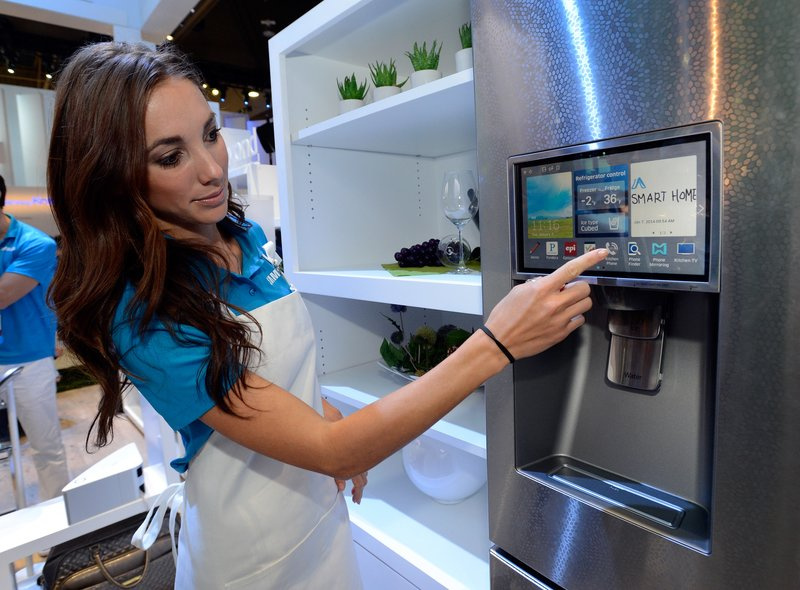
\includegraphics[scale=0.8]{imagens/geladeira.jpeg}}

    \footnotesize{Foto de David Becker, retirada do artigo de ~\citet{BajarinIoE2014}}%,
%      disponível em \url{http://time.com/539/the-next-big-thing-for-tech-the-internet-of-everything/}}
  \end{center}
\end{figure}

Se a IoT não se resume a eletrodomésticos conectados, o que ela é de fato? As
grandes empresas de tecnologia definem IoT do seguinte modo:

\begin{itemize}
\item \emph{\textbf{SAP}}: ``A Internet das Coisas é uma rede de objetos físicos --- veículos,
  máquinas, eletrodomésticos e outros --- que usam sensores e APIs para conectar e
  trocar dados na Internet''~\citep{SAPWhatIoT}.
\item \emph{\textbf{SAS}}: ``A Internet das Coisas é o conceito de objetos do cotidiano --- de
  máquinas industriais à dispositivos vestíveis ---- usando sensores embutidos para coletar
  dados e tomar uma ação sobre esses dados através da rede''\citep{SASWhatIoT}.
\item \emph{\textbf{IBM}}: ``A Internet das Coisas refere-se à variedade crescente
  de dispositivos conectados que enviam dados através da Internet. Uma 'coisa' é qualquer
  objeto com eletrônica embarcada que pode transferir dados em uma rede --- sem nenhuma
  interação humana''~\citep{IBMWhatIsIoT,IBMWhatsonIoT}.
\item \emph{\textbf{Cisco}}: ``A Internet das Coisas (IoT) refere-se simplesmente à conexão
  em rede de objetos físicos''~\citep{CiscoIoTVS2013}.
\item \emph{\textbf{Amazon}}: ``Um sistema de dispositivos ubíquos conectando o mundo
  físico à nuvem''~\citep{AmazonIoT}.
\item \emph{\textbf{Microsoft}}: embora a Microsoft não defina explicitamente o que
  ela entende por IoT, em um vídeo institucional sobre a plataforma \emph{Microsoft IoT}
  podemos deduzir que o conceito de IoT envolve conectar as partes mais vitais de
  seu negócio (pessoas, ativos, processos e sistemas), do chão de fábrica aos ``campos''
  para aumentar o alcançe da empresa e fazer melhor uso dos recursos~\citep{MicrosoftIoT}.
\item \emph{\textbf{Google}}: a empresa também não fornece uma definição explícita mas
  sua plataforma \emph{Google Cloud IoT Core} está voltada à ``conexão segura, coleta e
  gerenciamento de dados a partir de milhões de dispositivos globalmente dispersos [\ldots]
  para processar, analisar e visualizar dados em tempo real para suportar o aumento
  da eficiência operacional''~\citep{GoogleWhatsIoT}.
\end{itemize}

Um grande esforço de entendimento e conceituação da IoT foi realizado pelo \ingles{Institute
  of Electrical and Electronics Engineers (IEEE)} que, reconheceu a grande importância
do tema~\citep{IEEEIoTReport}, revisou a definição de IoT
de várias organizações, projetos de pesquisa, governos e instituições de ensino, e publicou
em 2015 sua própria definição de IoT no
relatório\footnote{\url{https://iot.ieee.org/definition.html}}\textsuperscript{, }\footnote{O IEEE revisou
  as definições e conceituações de IoT de 8 organismos internacionais de padronização, 8 projetos
  de pesquisa em IoT, 3 iniciativas de governos, 7 relatórios institucionais de empresas e
  consultorias, 5 livros que tratam exclusivamente de IoT e 3 definições fornecidas por indústrias
que lidam com IoT.}
``\ingles{Towards a definition of
  the Internet of Things (IoT)}''~\citep{IEEEIoTDefinition}. A definição proposta
pelo IEEE é a seguinte:

\begin{quote}
  ``A Internet das Coisas (IoT) é uma rede complexa, auto-configurá-vel e adaptativa,
  que interconecta 'coisas' à Internet através do uso de protocolos de comunicação
  padronizados. As coisas interconectadas têm representação física ou virtual no mundo
  digital, com capacidades sensoriais, de atuação e programabilidade, e são unicamente
  identificáveis. A representação contém informação sobre a coisa incluindo sua identidade,
  status, localização ou qualquer outra informação relevante, privada, social ou
  empresarial. A coisa oferece serviços, com ou sem a intervenção humana, através
  da exploração de sua identificação única, dados capturados, comunicação e capacidade
  de atuação. Os serviços são explorados através do uso de interfaces inteligentes e
  estão disponíveis em qualquer lugar, a qualquer hora e para qualquer um ou qualquer
  coisa, levando em consideração questões de segurança.''~\citep{IEEEIoTDefinition}
\end{quote}

Dissecando a definição da IEEE podemos compreender melhor cada parte da IoT:

\begin{enumerate}
\item \emph{\textbf{Coisa}}: é qualquer dispositivo que possa ser conectado
  à Internet, variando desde um minúsculo sensor até um carro ou outro
  grande equipamento, e que tenha capacidade sensorial, de atuação ou de
  programabilidade.
\item \emph{\textbf{Identificação única}}: cada coisa deve ser unicamente
  identificável na Internet pois só assim pode-se captar dados relevantes
  e oferecer serviços importantes para cada um.
\item \emph{\textbf{Ubiquidade}}: as coisas e os serviços por elas disponibilizados
  devem estar disponíveis em qualquer lugar, a qualquer hora e para qualquer um
  ou qualquer coisa (note-se que uma coisa pode oferecer serviços para outras
  coisas).
\item \emph{\textbf{Rede}}: as coisas conversam, trocam dados e oferecem
  serviços através de uma rede complexa, atualmente a Internet.
\item \emph{\textbf{Autonomia}}: as coisas devem ser capazes de
  obter dados e oferecer serviços sem a intervenção humana (não excluindo
  a possibilidade da participação humana ativa também).
\item \emph{\textbf{Segurança}}: toda essa atividade de coleta e troca de
  dados via rede resulta em desafios imensos relacionados à segurança e
  privacidade das informações, e as questões de segurança devem ser
  tratadas pelas coisas e seus protocolos de comunicação.
\end{enumerate}


%%%%%%%%%%%%%%%%%%%%%%%%%%%%%%%%%%%%%%%%%%%%%%%%%%%%%%%%%%%%%%%%%%%%%%%%%%%%%%%%%
%%%%%%%%%%%%%%%%%%%%%%%%%%%%%%%%%%%%%%%%%%%%%%%%%%%%%%%%%%%%%%%%%%%%%%%%%%%%%%%%%
\subsection{Ecossistema da IoT}
\label{o-que-e-iot-ecossistema}

Todas as ``coisas'' conectadas à internet, incluindo todo o \ingles{hardware}
e \ingles{software} formam o ``ecossistema da IoT'' (ver Figuras~\ref{fig:ecossistema1}
e \ref{fig:ecossistema2}).

O \ingles{hardware} inclui os próprios dispositivos, sensores, atuadores,
servidores de processamento, servidores de armazenamento de dados,
infra-estrutura de rede, infra-estrutura de nuvem, equipamentos de backup, etc. Enfim,
inclui tudo o que é necessário para manter a estrutura da IoT funcionando.

O \ingles{software} inlcui os sistemas embarcados nos dispositivos, os sistemas
nos servidores, os sistemas de coleta e análise de dados ou qualquer outro
sistema ou programa para que a IoT funcione adequadamente.

\begin{figure}[h]
  \begin{center}
    \caption{Ecossistema, características e escopo da IoT.}
    \label{fig:ecossistema1}
    \fbox{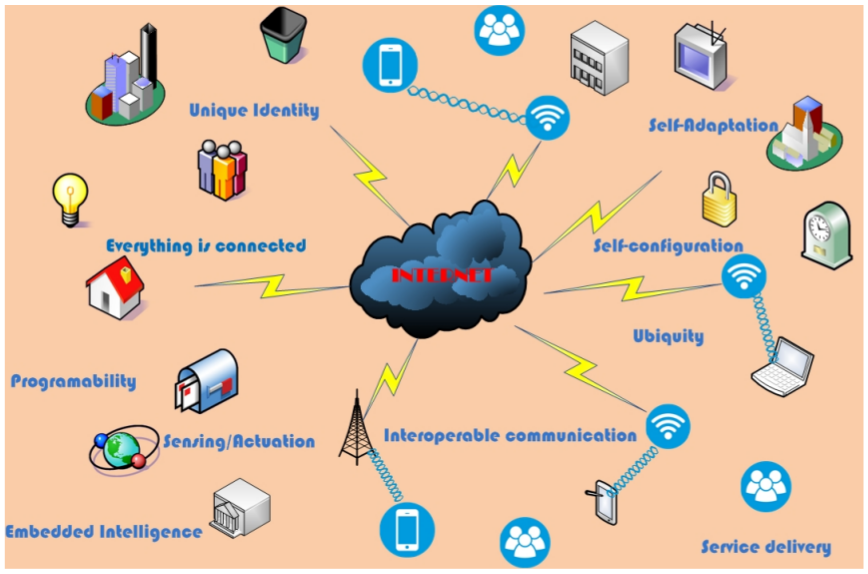
\includegraphics[scale=0.4]{imagens/ecossistema1.png}}
    
    \footnotesize{Ilustração retirada do relatório do~\citet{IEEEIoTDefinition}}
  \end{center}
\end{figure}

\begin{figure}[h]
  \begin{center}
    \caption{Ecossistema da IoT.}
    \label{fig:ecossistema2}
    \fbox{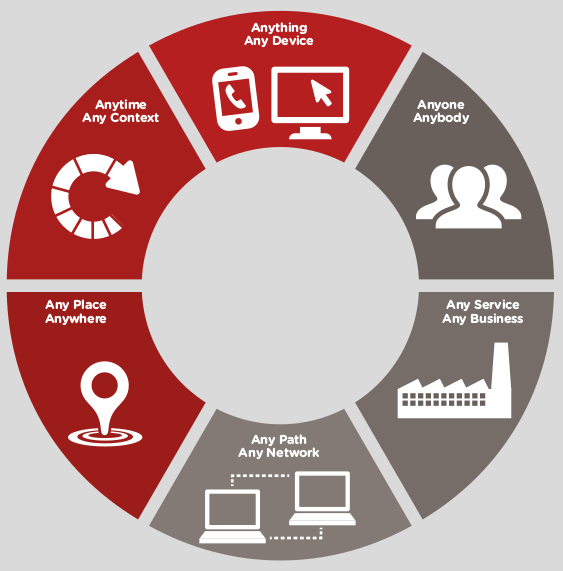
\includegraphics[scale=0.5]{imagens/ecossistema2.png}}
    
    \footnotesize{Ilustração retirada do relatório de~\citet{UKGOSWalportIoT2014}}
  \end{center}
\end{figure}

Alguns autores~\citep{UKGOSWalportIoT2014,IEEEIoTDefinition,BarbozaTCCIoT2015}
identificam, a grosso modo, dois ``tamanhos'' de ecossistema para as aplicações da IoT:
pequena ou grande escala. O que diferencia entre essas duas é a comlexidade em termos
de:

\begin{itemize}[noitemsep]
\item Número de dispositivos
\item Propriedade e gerenciamento das coisas
\end{itemize}

Um ecossistema IoT de pequena escala corresponde à uma rede de dispositivos
pouco complexa, com relativamente poucos dispositivos e, principalmente, com
um único proprietário gerenciador. Aqui se encaixam as soluções
de IoT de um único fabricante. Por exemplo: sistemas para a irrigação de jardins
que utilizam dados de previsão do tempo, sistemas em veículos que indicam ao
motorista a necessidade de manutenção preventiva, sistemas em marca-passos cardíacos
que avisam à equipe médica se algum problema ocorrer.

Por outro lado, um ecossistema IoT de grande escala corresponde à uma rede
de dispositivos muito complexa, com muitos dispositivos e, principalmente, com
diversos proprietários e gerenciadores (que podem até não ter relacionamentos
explícitos entre eles). Segundo o \citet{IEEEIoTDefinition}, ``nesse contexto,
a complexidade torna-se dominante e elementos como escalabilidade, lógica distribuída,
etc., tornam-se essenciais. Todas as abordagens tradicionais para gerenciamento
de confiança, nomeação, descoberta, etc., devem ser completamente repensadas''.

As soluções de pequena escala, apesar do nome, já causam profundo impacto na sociedade
mas o maior potencial para a IoT será quando for possível conectar todos os dispositivos,
de todos os fabricantes, em um ecossistema de grande escala~\citep{UKGOSWalportIoT2014,IEEEIoTDefinition,BhattIoT,IEEEIoTReport,McKinseyIoTHype,MoolayilIoT2016,RajIoT2017,OliverWymanIoT2015,SAPFutureIoT,CiscoIoEPublicSectorOpportunity,CiscoIoTFAQ2013,CiscoIoTVS2013,CiscoIoEPublicSectorEconomicAnalysis,CiscoIoESurvey2013,CiscoIoEValuePrivate2013,CiscoIoEValuePublic2013}.

Obviamente, apesar do grande potencial em conectar todos os dispositivos, de todos
os fabricantes, em uma grande rede comum de troca de informações e prestação de
serviços, existem grandes obstáculos a serem superados até que essa visão de futuro
possa ser alcançada \citep{UKGOSWalportIoT2014}.


%%%%%%%%%%%%%%%%%%%%%%%%%%%%%%%%%%%%%%%%%%%%%%%%%%%%%%%%%%%%%%%%%%%%%%%%%%%%%%%%%
%%%%%%%%%%%%%%%%%%%%%%%%%%%%%%%%%%%%%%%%%%%%%%%%%%%%%%%%%%%%%%%%%%%%%%%%%%%%%%%%%
\subsection{Breve histórico}
\label{o-que-e-iot-historia}

Pode-se afirmar que a história da IoT está intimamente ligada ao desenvolvimento
da tecnologia de \ingles{Radio-Frequency Identification (RFID)}, cujas raízes
tecnológicas podem ser verificáveis desde a segunda guerra mundial~\citep{IEEEIoTDefinition}.
Os países em guerra já utilizavam radares para detectar a aproximação de aviões,
mas não existia um jeito de dizer se os aviões eram de inimigos se aproximando
ou se eram aviões amigos retornando de uma missão. Os alemães foram os
primeiros a descobrir que, se os pilotos executassem manobras de ``rolamento''
com os aviões, isso alterava o sinal do radar e permita aos operadores em terra
saber se os aviões eram alemães ou se eram aviões inimigos. Essencialmente
isso era o primeiro sistema de RFID passivo.

Os britânicos logo desenvolveram um sistema ativo de identificação: quan-do
um avião britânico recebia um sinal de radares britânicos, ele repondia através
do \emph{broadcast} de um sinal que era percebido pelos operadores em terra
como um avião amigo~\citep{IEEEIoTDefinition}.

Segundo o~\citet{IEEEIoTDefinition} a tecnologia RFID funciona basicamente
através do mesmo conceito: ``um sinal é enviado a um tipo de \emph{transponder}
que 'acorda' e ou reflete de volta (RFID passivo) ou realiza
um \emph{broadcast} (RFID ativo) de um sinal''.

Após a guerra, durante as décadas de 1950 e 1960, cientistas e acadêmicos
continuaram a desenvolver tecnologias de rádio-freqüência para identificar
objetos remotamente. Empresas começaram a comercializar sistemas anti-furto
que funcionavam com uma \ingles{tag} eletrônica capaz de informar se o produto
foi pago ou não. Esse sitema, em uso ainda hoje, é composto por \ingles{tags}
que armazenam apenas 1 \ingles{bit} --- 0 (o produto foi pago) ou 1 (o produto não
foi pago) --- e leitores de rádio-freqüência que são instalados nas portas
das lojas~\citep{IEEEIoTDefinition}.

Outros avanços importantes da área de identificação por rádio-freqüência, que
contribuíram para o desenvolvimento da IoT, foram:

\begin{itemize}
\item \emph{RFID ativo com memória regravável}: a primeira patente de um sistema de RFID ativo,
  com memória regravável foi obtida por Mario W. Cardullo, em 1973. Maiores informações
  sobre essa tecnologia podem ser encontradas no artigo de \citet{CardulloRFIDGenesis2003}.
\item \emph{Cartões fechadura}: também em 1973, Charles Walton desenvolveu um sistema
  de cartões plásticos com \ingles{transponders RFID} embutidos, capazes de abrir
  portas sem a necessidade de chaves~\citep{IEEEIoTDefinition}. Esse sistema é
  utilizado ainda hoje em hotéis, por exemplo.
\item \emph{Sistemas automáticos de pagamento de pedágio}: durante a década de 1970,
  cientistas do \emph{Los Alamos National Laboratory} desenvolveram uma tecnologia
  para rastrear o transporte de manterial de bombas nucleares, usando RFIDs com
  capacidade de armazenar maiores informações. Em 1980 esses mesmos cientistas
  fundaram uma empresa e passaram a vender essa tecnologia, agora voltada
  para uso civil, em um sistema de pagamento automático de pedagios (que está em uso
  até hoje)~\citep{IEEEIoTDefinition}.
\item \emph{Rastreamento de gado}: os cientistas do \emph{Los Alamos National Laboratory}
  também desenvolveram um sistema de rastreamento e identificação única voltado
  para gado, para monitorar a localização dos animais e as doses de hormônios e
  vacinas que eles já tinham recebido~\citep{IEEEIoTDefinition}.
\end{itemize}

Pela lista acima podemos ver que a aplicação da tecnologia RFID foi sendo
expandida: não servia mais só para identificar um objeto, mas também armazenar
dados sobre esse mesmo objeto. Isso era um grande avanço, mas gerava um problema:
armazenar diversos dados em uma \ingles{tag} RFID levava ao aumento do custo
unitário. A idéia era boa, mas era necessário alguma inovação que barateasse o
sistema. Essa inovação começou a surgir em 1990: no início da década de 1990
a IBM patenteou um sistema de \emph{Ultra-High Frequency} (UHF) RFID, tornando
possível que a leitura dos dados da \emph{tag} fosse feita a uma distância maior
do que até então era possível e com uma rápida velocidade de
transferência~\citep{IEEEIoTDefinition}.

Em 1999 foi fundado, no \ingles{Massachusetts Institute of Technology (MIT)}, um
laboratório de inovação chamado de \emph{Auto-ID Center}, cujo objetivo era
desenvolver inovação na área de identificação por rádio-freqüência baseando-se
na tecnologia de UHF RFID desenvolvida pela IBM. Dois cientistas do \ingles{Auto-ID Center},
David Brock e Sanjay Sarma, foram os pioneiros em investigar a possibilidade
de usar \ingles{tags} UHF RFID de baixo custo em todos os produtos da cadeia
de suprimento. A idéia deles era colocar apenas o número de série de cada produto
na \ingles{tag}, barateando seu custo, e manter os dados detalhados de cada
produto em um banco de dados que seria acessível pela Internet~\citep{IEEEIoTDefinition}.
\textbf{Assim nasceu a conexão das coisas com a Internet}.

Para Roberti, citado em \citet{IEEEIoTDefinition}:
\begin{quote}
``Sarma e Brock
essencialmente mudaram a maneira como as pessoas pensavam sobre o RFID na
cadeia de suprimentos. Antes, as \ingles{tags} eram um banco de dados móvel
que carregavam informações sobre o produto à medida em que esse produto
seguia seu curso. Sarma e Brock \textbf{tornaram o RFID em uma tecnologia de rede
  através da ligação de objetos com a Internet através das \ingles{tags}}.'' [grifos
  nossos]
\end{quote}

A criação do termo \ingles{Internet of Things (IoT)} é atualmente creditada à Kevin Ashton,
na época o diretor executivo do \ingles{Auto-ID Center}, mas existe uma certa
controvérsia quanto a isso pois segundo Daniel Engels (também um dos
diretores), citado por~\citet{IEEEIoTDefinition},
o termo foi usado pela primeira vez em 1997 em uma publicação da
\ingles{International Telecommunication Union (ITU)}, e Kevin Ashton disse
que cunhou o termo em 1999~\citep{AshtonIoT2009,PressIoT2014}.


%%%%%%%%%%%%%%%%%%%%%%%%%%%%%%%%%%%%%%%%%%%%%%%%%%%%%%%%%%%%%%%%%%%%%%%%%%%%%%%%%
%%%%%%%%%%%%%%%%%%%%%%%%%%%%%%%%%%%%%%%%%%%%%%%%%%%%%%%%%%%%%%%%%%%%%%%%%%%%%%%%%
\subsection{Outros tipos de ``internet das coisas''}
\label{o-que-e-iot-outros-tipos}

É importante salientar que exitem outros termos e tecnologias relacionadas à
IoT que tratam de coisas semelhantes. Esses outros termos às vezes são usados
como sinônimos de IoT, outras vezes como complementares ou referentes a uma
parte específica do ecossistema da IoT, causando uma certa confusão. Esta
seção explicará brevemente os principais termos alternativos, sem entrar em
maiores detalhes de cada um pois isso foge ao escopo deste trabalho.


%%%%%%%%%%%%%%%%%%%%%%%%%%%%%%%%%%%%%%%%%%%%%%%%%%%%%%%%%%%%%%%%%%%%%%%%%%%%%%%%%
\subsubsection{\ingles{Internet of Everything (IoE)}}
\label{o-que-e-iot-outros-tipos-ioe}

Alguns autores e empresas fazem uma diferenciação entre a \ingles{Internet of Things (IoT)}
e a \ingles{Internet
  of Everything (IoE)}, sendo esta ``a conexão em rede de pessoas, processos,
dados e coisas'', e aquela ``simplesmente a conexão em rede de coisas
e dados''~\citep{CiscoIoEPublicSectorOpportunity,CiscoIoTVS2013,CiscoIoTFAQ2013}.
Assim, a IoE é uma ``evolução'' da IoT, cujo escopo e potencial
são maiores. Segundo \citet{HebraIoTIoE2015} o futuro da IoT caminha para
ser a IoE, trazendo enormes vantagens e benefícios.

A IoE seria uma maneira de incluir tudo o que pode ser conectado, não apenas
coisas e dados, mas algo bem maior e global~\citep{LuethIoT2014,BajarinIoE2014}.


%%%%%%%%%%%%%%%%%%%%%%%%%%%%%%%%%%%%%%%%%%%%%%%%%%%%%%%%%%%%%%%%%%%%%%%%%%%%%%%%%
\subsubsection{\ingles{Machine-to-Machine (M2M) Communication}}
\label{o-que-e-iot-outros-tipos-m2m}

Segundo~\citet{IEEEIoTDefinition}, ``a comunicação máquina-a-máquina (M2M) é a
comunicação entre duas ou mais entidades do mesmo tipo que não precisam necessariamente de nenhuma
intervenção humana direta. Serviços de M2M pretendem automatizar deicões
e processos de comunicação''.

Para~\citet{LuethIoT2014}, ``o termo comunicação máquina-a-máquina (M2M) está em
uso há mais de uma década e é bem conhecido no setor de telecomunicações. Inicialmente
a comunicação M2M era uma conexão um-a-um, fazendo a ligação entre uma máquina e outra.
Mas hoje, com a explosão da conectividade móvel, dados são mais facilmente transmitidos
via um sistema de rede IP, e muitos outros dispositivos participam da comunicação''.


%%%%%%%%%%%%%%%%%%%%%%%%%%%%%%%%%%%%%%%%%%%%%%%%%%%%%%%%%%%%%%%%%%%%%%%%%%%%%%%%%
\subsubsection{\ingles{Industrial Internet of Things (IIoT)}}
\label{o-que-e-iot-outros-tipos-iiot}

É um termo mais abrangente que a M2M pois envolve, não apenas a comunicação
máquina-a-máquina, mas também a comunicação com interfaces humanas \citet{LuethIoT2014}
integrando máquinas complexas com software e sensores em rede.


%%%%%%%%%%%%%%%%%%%%%%%%%%%%%%%%%%%%%%%%%%%%%%%%%%%%%%%%%%%%%%%%%%%%%%%%%%%%%%%%%
\subsubsection{\ingles{Web of Things (WoT)}}
\label{o-que-e-iot-outros-tipos-wot}

Segundo \citet{LuethIoT2014}, a \ingles{Web of Things} ``é um conjunto de
arquitetura de \ingles{software} e padrões de programação que permitem que
objetos do mundo real façam parte da \ingles{world wide web}''. É assim um conceito
mais estreito do que a IoT pois está focado somente em \ingles{software}.


%%%%%%%%%%%%%%%%%%%%%%%%%%%%%%%%%%%%%%%%%%%%%%%%%%%%%%%%%%%%%%%%%%%%%%%%%%%%%%%%%
\subsubsection{\ingles{Industry 4.0}}
\label{o-que-e-iot-outros-tipos-industry-4.0}

O temo \ingles{Industry 4.0} ``descreve um conjunto de conceitos que pretendem
direcionar a próxima revolução industrial, incluindo todos os tipos de conceitos
de conectividade em um contexto industrial, indo além e incluindo mudanças reais
no mundo físico tais como o uso de tecnologias de impressão 3D ou o uso de realidade
virtual ou aumentado no processo de industrialização''~\citet{LuethIoT2014}.


%%%%%%%%%%%%%%%%%%%%%%%%%%%%%%%%%%%%%%%%%%%%%%%%%%%%%%%%%%%%%%%%%%%%%%%%%%%%%%%%%
\subsubsection{O conjunto dos outros tipos de ``internet das coisas''}
\label{o-que-e-iot-outros-tipos-conjunto}

Uma figura esquemática simples e objetiva do que é cada tipo de internet das coisas
discutida nesta seção é fornecida por ~\citet{LuethIoT2014}. Nesse esquema
(ver Figura~\ref{fig:outras-iot}) pode-se
perceber de maneira objetiva o escopo de cada tecnologia e como cada uma se relaciona
com as outras.

\begin{figure}[h]
  \begin{center}
    \caption{Relações entre IoT, IoE, M2M, IIoT, WoT e Indústria 4.0}
    \label{fig:outras-iot}
    \fbox{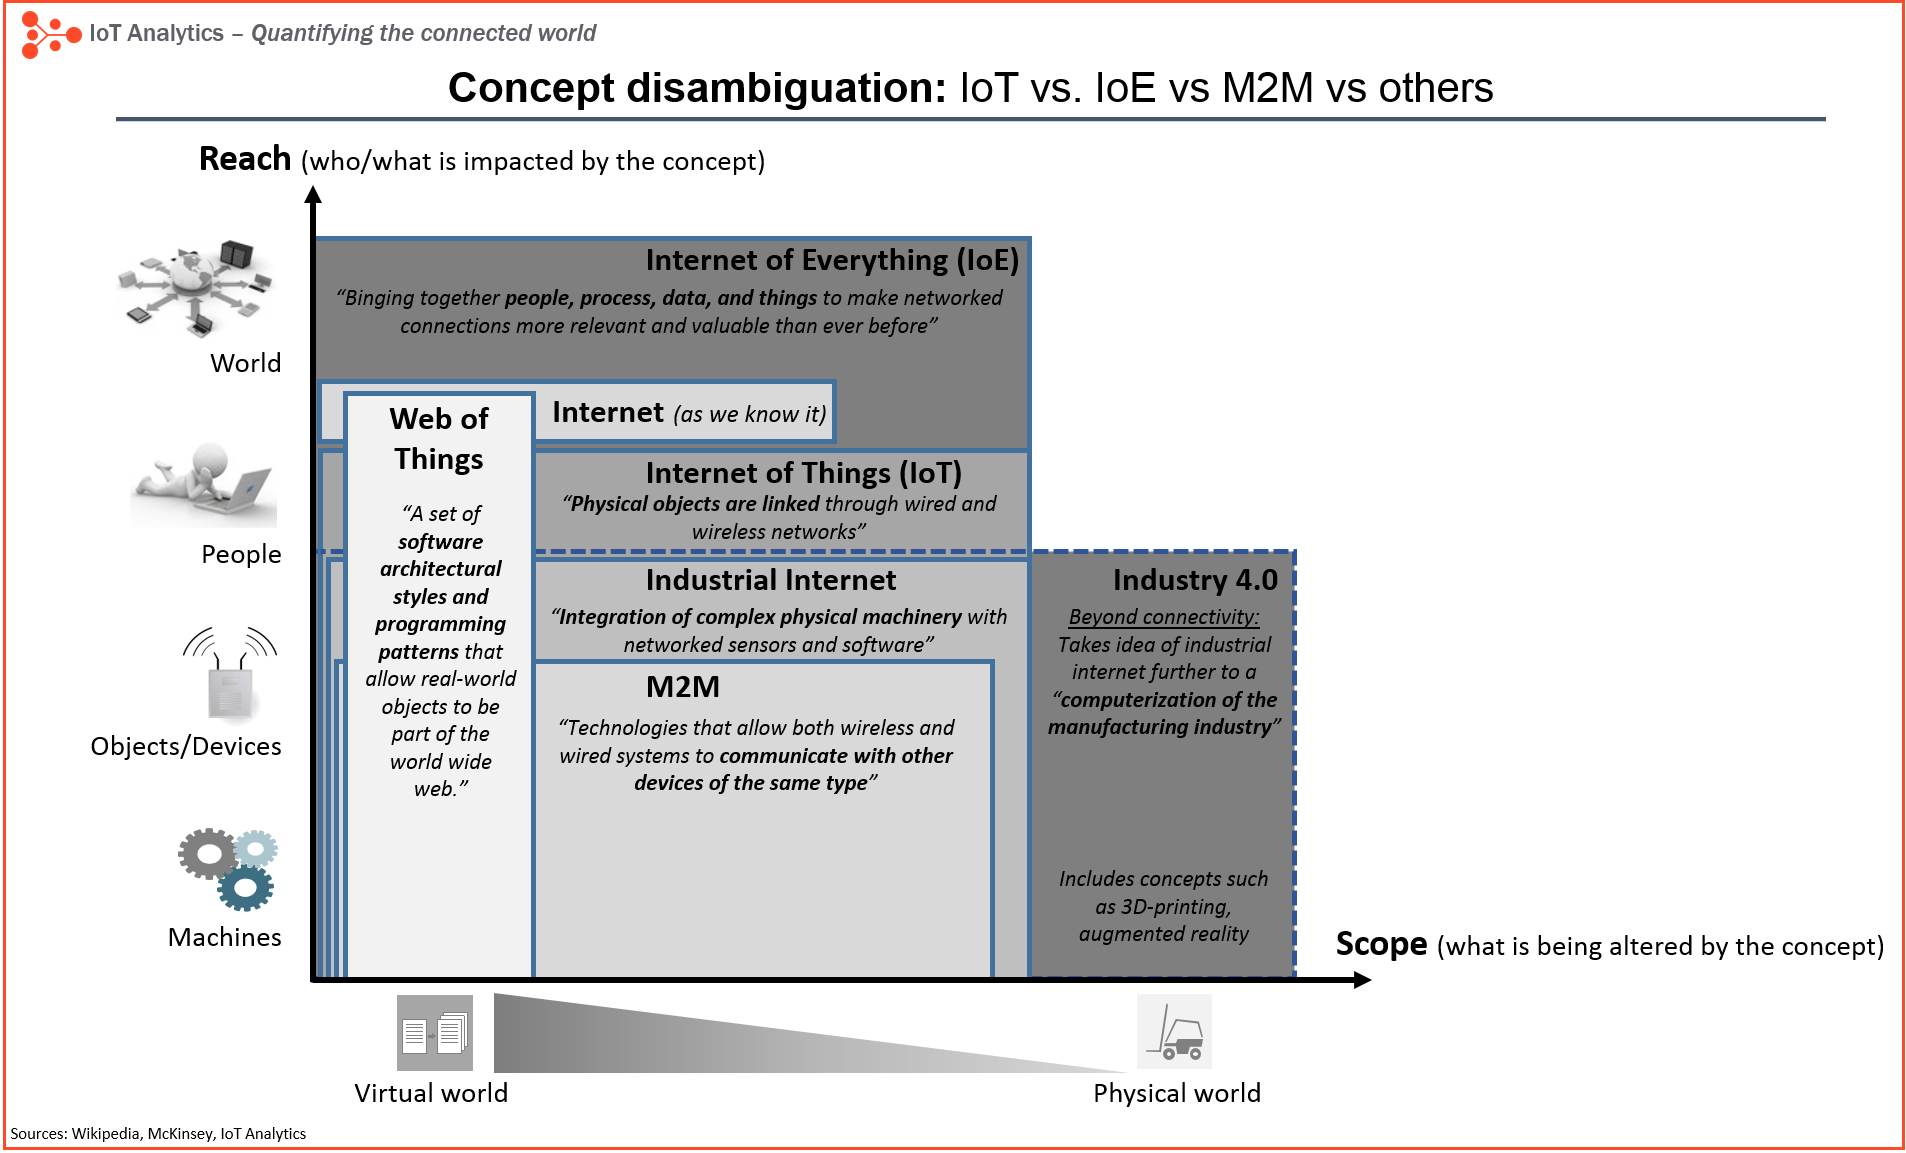
\includegraphics[scale=0.21]{imagens/outras-iot.png}}
    
    \footnotesize{Ilustração retirada de~\citet{LuethIoT2014},
      disponível em \url{https://iot-analytics.com/internet-of-things-definition/}.}
  \end{center}
\end{figure}


%%%%%%%%%%%%%%%%%%%%%%%%%%%%%%%%%%%%%%%%%%%%%%%%%%%%%%%%%%%%%%%%%%%%%%%%%%%%%%%%%
%%%%%%%%%%%%%%%%%%%%%%%%%%%%%%%%%%%%%%%%%%%%%%%%%%%%%%%%%%%%%%%%%%%%%%%%%%%%%%%%%
%%%%%%%%%%%%%%%%%%%%%%%%%%%%%%%%%%%%%%%%%%%%%%%%%%%%%%%%%%%%%%%%%%%%%%%%%%%%%%%%%
\section{Aplicações da IoT}
\label{aplicacoes-iot}

Sem dúvida nenhuma as áreas onde a IoT pode ser aplicada são limitadas apenas
pela imaginação humana, variando desde um simples eletrodoméstico até grandes
sistemas industriais ou sistemas para cidades inteiras.

O potencial é tão grande que ``é impossível antecipar
todas as mudanças sociais que podem ser criadas atraves da conexão de bilhões
de dispositivos''~\citep{UKGOSWalportIoT2014}.

De modo geral os autores~\citep{OliverWymanIoT2015,UKGOSWalportIoT2014,IEEEIoTReport,IEEEIoTDefinition,ChuiIoT2010,BughinExecutiveIoT2015,GuptaMcKinseyIoT2017,McKinseyIoTHype,SAPFutureIoT,SASIoTUseCases2016} citam as seguintes grandes
áreas como as que mais se beneficiarão da aplicação da IoT (ver também
Figuras~\ref{fig:aplicacoes-iot-1}, \ref{fig:aplicacoes-iot-2} e \ref{fig:aplicacoes-iot-3}):

\begin{itemize}[noitemsep]
\item Saúde
\item Agricultura
\item Construção civil (incluindo os lares)
\item Varejo
\item Energia, petróleo, gás e mineração
\item Indústria
\item Mobilidade e transporte (incluindo veículos autônomos)
\item Logística
\item Mídia
\item Cidades inteligentes
\end{itemize}

\begin{figure}[!h]
  \begin{center}
    \caption{Principais aplicações da IoT, segundo~\citet{OliverWymanIoT2015}}
    \label{fig:aplicacoes-iot-1}
    \fbox{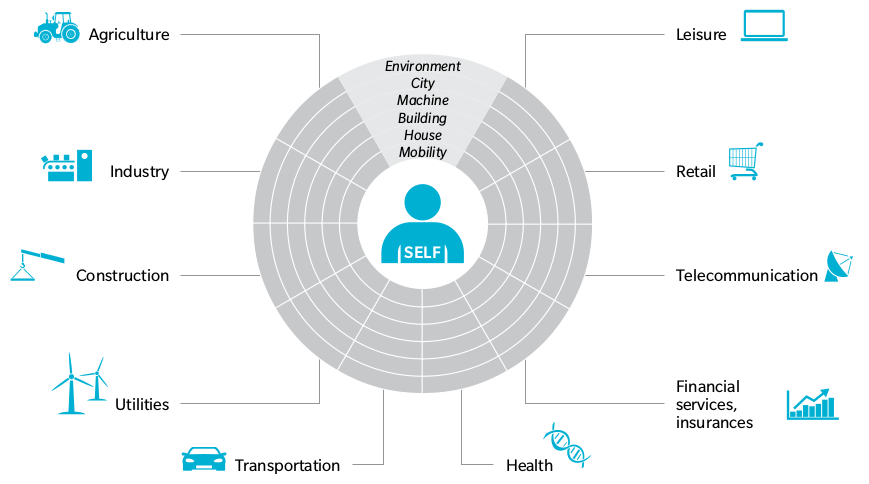
\includegraphics[scale=0.4]{imagens/aplicacoes-1.png}}
    
    \footnotesize{Ilustração retirada de~\citet{OliverWymanIoT2015}}
  \end{center}
\end{figure}

\begin{figure}[!h]
  \begin{center}
    \caption{Principais setores beneficiados pela IoT e seus \ingles{stakeholders}
      mais importantes, segundo o~\citet{IEEEIoTDefinition}}
    \label{fig:aplicacoes-iot-2}
    \fbox{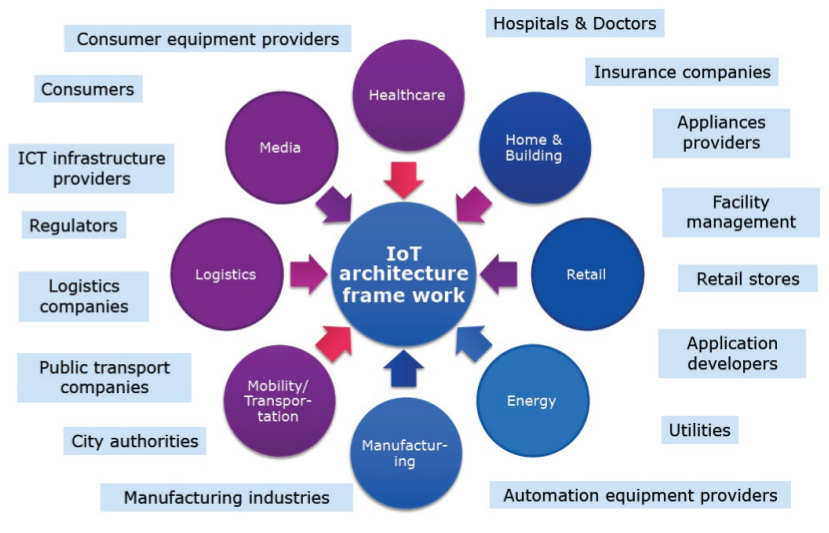
\includegraphics[scale=0.4]{imagens/aplicacoes-2.png}}
    
    \footnotesize{Ilustração retirada de~\citet{IEEEIoTDefinition}}
  \end{center}
\end{figure}

\begin{figure}[!h]
  \begin{center}
    \caption{Principais áreas de aplicação da IoT, segundo~\citet{McKinseyIoTHype}}
    \label{fig:aplicacoes-iot-3}
    \fbox{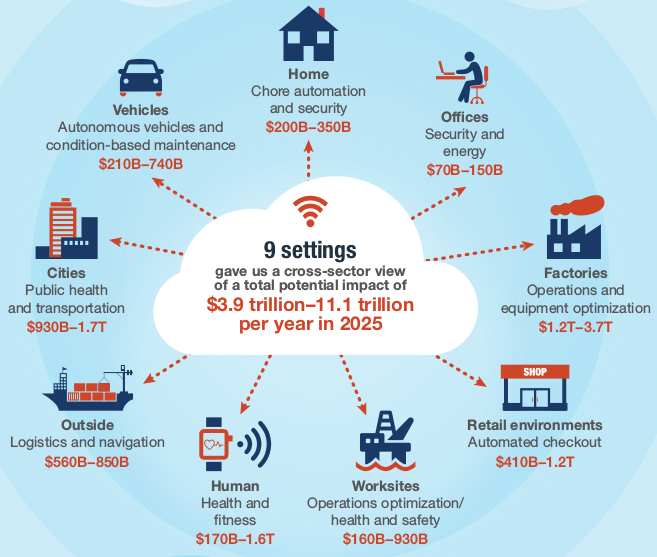
\includegraphics[scale=0.4]{imagens/aplicacoes-3.png}}
    
    \footnotesize{Ilustração retirada de~\citet{McKinseyIoTHype}}
  \end{center}
\end{figure}

As próximas seções detalharão como a IoT causará um impacto benéfico, e mostrarão
alguns casos de sucesso que ilustram todo o potencial dessa nova tecnologia.


%%%%%%%%%%%%%%%%%%%%%%%%%%%%%%%%%%%%%%%%%%%%%%%%%%%%%%%%%%%%%%%%%%%%%%%%%%%%%%%%%
%%%%%%%%%%%%%%%%%%%%%%%%%%%%%%%%%%%%%%%%%%%%%%%%%%%%%%%%%%%%%%%%%%%%%%%%%%%%%%%%%
\subsection{Como a IoT cria valor?}
\label{aplicacoes-iot-criacao-valor}

Antes de discutirmos casos concretos da aplicação da IoT, é importante ter clara
a noção de como a IoT cria valor, ou seja, como uma rede de coisas conectadas
podem beneficiar as pessoas e gerar valor para elas e para as empresas.

\citet{ChuiIoT2010} classifica o mecanismo de geração de valor da IoT em
dois grandes grupos: um grupo de \textbf{Informação e Análise} (que envolve atividades
de monitoramento de comportamento, obtenção de consciência em tempo real do ambiente
físico e a tomada de decisões baseadas em \emph{analytics} de sensores) e
um grupo de \textbf{Automação e Controle} (que envolve atividades de otimização
de processos, otimização do consumo de recursos e o desenvolvimento de sistemas
autônomos complexos).

Explicando melhor como a IoT gera valor, \citet{ChuiIoT2010} nos fornece
as seguintes informações:

\begin{itemize}
\item \emph{\textbf{Informação e Análise}}: a IoT pode fornecer mais e melhor
  informação e análise, aumentando a velocidade e a performance da tomada de
  decisão. Isso é obtido através de:
  \begin{itemize}
  \item \emph{Monitoramento de comportamento}: inclui as atividades
    de monitoramento do comportamento, status e outras variáveis de pessoas,
    coisas ou dadados, no espaço e tempo. Por exemplo: uma empresa de seguros
    pode colocar sensores em carros e monitorar como e por onde um carro trafega,
    podendo basear políticas de preços personalizadas com essa informação; empresas
    podem monitorar a movimentação de produtos por toda a cadeia de suprimentos,
    melhorando o controle de estoque e reduzindo perdas.
  \item \emph{Obter consciência em tempo real do ambiente físico}: inclui as
    atividades que visam obter dados, em tempo real, de sensores alocados em
    diversas coisas ou lugares, para fornecer aos tomadores de decisão uma visão
    em tempo real do ambiente. Por exemplo: sensores sônicos espalhados pela cidade
    podem fornecer às delegacias de polícia dados instantâneos sobre a localização
    em tempo real de disparos de arma de fogo.
  \item \emph{Decisões orientadas por} analytics \emph{baseada em sensores}: a
    obtenção de dados em tempo real e sua ligação à sistema de análises automatizados
    pode orientar decisões humanas ou automáticas em diversos serviços e áreas de
    aplicação. Por exemplo: varejistas podem monitorar através de sensores a
    movimentação de clientes pela loja, verificando quais produtos os clientes
    gastam mais tempo observando, e disparar promoções ou propagandas imediatas.
  \end{itemize}
\item \emph{\textbf{Automação e Controle}}: a IoT pode criar uma base para
  automação e controle convertendo os dados obtidos pelos sensores em \emph{feedback}
  para os atuadores para a otimização e ajuste de diversos processos. Isso é obtido
  através de:
  \begin{itemize}
  \item \emph{Otimização de processos}: inclui as atividades que visam obter
    de sensores informações importantes sobre processos, analisá-las automaticamente
    e ajustar o processo para otimizá-lo em tempo real. Por exemplo: uma indústria
    pode instalar sensores de temperatura para manter sempre na faixa adequada
    um forno utilizado na produção.
  \item \emph{Otimização do consumo de recursos}: inclui as atividades que podem
    auxiliar a mudar e otimizar o uso de recursos, incluindo energia, água e
    demais recursos. Por exemplo: uma empresa de energia pode fornecer medidores
    de consumo elétrico que mostram, em tempo real, o consumo e o custo imediato
    de fornecimento, cobrando diferentemente pelo padrão e horário de uso.
  \item \emph{Sistemas autônomos complexos}: inclui as atividades que envolvem
    a rápida detecção em tempo real de condições imprevisíveis e respostas
    instantâneas guiadas por sistemas automáticos que imitam as reações humanas
    (e escolhem a melhor reação entre várias possíveis). Por exemplo: montadoras
    estão desenvolvendo vários tipos de sistemas de caros, desde sistemas de
    detecção e evasão de colisões, até carros autônomos.
  \end{itemize}
\end{itemize}

Enfim, as possibilidades de geração de valor com a IoT são enormes e, à medida
em que usos mais inteligentes e inovadores dos sensores e dos dados obtidos forem
desenvolvidos, outros modelos de negócios e formas de geração de valor serão
criados e implementados.


%%%%%%%%%%%%%%%%%%%%%%%%%%%%%%%%%%%%%%%%%%%%%%%%%%%%%%%%%%%%%%%%%%%%%%%%%%%%%%%%%
%%%%%%%%%%%%%%%%%%%%%%%%%%%%%%%%%%%%%%%%%%%%%%%%%%%%%%%%%%%%%%%%%%%%%%%%%%%%%%%%%
\subsection{Exemplos atuais de aplicação da IoT}
\label{aplicacoes-iot-exemplos}

Devido às inúmeras aplicações da IoT já citadas na Seção~\ref{aplicacoes-iot},
apresentaremos aqui apenas alguns exemplos em três áreas: cuidados de saúde,
agricultura e transporte. Diversos outros exemplos podem ser obtidos consultando-se
as referências bibliográficas indicadas\footnote{\citet{OliverWymanIoT2015,UKGOSWalportIoT2014,IEEEIoTReport,IEEEIoTDefinition,ChuiIoT2010,BughinExecutiveIoT2015,GuptaMcKinseyIoT2017,McKinseyIoTHype,SAPFutureIoT,SASIoTUseCases2016,MorganStanleyIoTnow2013,AlaskaIoTComm2015,BackDeckerIoT2014,MazakIoT2016,CopenhagenIoT2013,KansasIoT2016,RockwellIoT2016,MississaugaIoT2015}}.


%%%%%%%%%%%%%%%%%%%%%%%%%%%%%%%%%%%%%%%%%%%%%%%%%%%%%%%%%%%%%%%%%%%%%%%%%%%%%%%%%
\subsubsection{Cuidados de saúde}
\label{aplicacoes-iot-exemplos-saude}

Segundo \citet{UKGOSWalportIoT2014} a IoT nos cuidados de saúde ``pode ajudar
a mudar o foco da cura para a prevenção e dar às pessoas maior controle sobre
as decisões que afetam seu bem-estar''. Algumas aplicações já existem:

\paragraph{Ambulâncias aéreas} A \ingles{California Shock Trauma Air Rescure (CALSTAR)}
é um serviço de ambulância aérea que começou a utilizar conceitos de IoT para
integrar sistemas de comunicação ar-solo para conectar suas aeronavas de
transporte às instituições de saúde~\citep{CiscoCALSTAR}.

\paragraph{Aplicativos \emph{fitness}} Diversos aplicativos voltados para saúde
e \emph{fitness} já existem, alguns conectados à sensores IoT que captam
dados como freqüência cardíaca. Os dez maiores aplicativos desse gênero
estão realmente contribuindo para tornar mais saudáveis os hábitos
de saúde de seus usuários~\citep{OliverWymanIoT2015}.

\paragraph{Monitoramento contínuo} Usando soluções de monitoramento contínuo,
a IoT está aumentando a aderência dos pacientes às terapias prescritas, diminuindo
as internações e aumentanto a qualidade de vida de pacientes~\citep{McKinseyIoTHype}.


%%%%%%%%%%%%%%%%%%%%%%%%%%%%%%%%%%%%%%%%%%%%%%%%%%%%%%%%%%%%%%%%%%%%%%%%%%%%%%%%%
\subsubsection{Agricultura}
\label{aplicacoes-iot-exemplos-agricultura}

Aplicações da IoT na área de agricultura são diversas e com potencial de aumentar
a produtividade alimentar e aumentar a proteção ao meio ambiente. Algumas
iniciativas interessantes:

\paragraph{Monitoramento de colméias} Soluções de IoT já são utilizadas para
monitorar colméias de abelhas em tempo real, reduzindo a inspeção manual que causa
distúrbios nas colméias e diminuem a produtividade de mel~\citep{SilvaIoTColmeia2017}.

\paragraph{Sistemas de irrigação} Já existem sistemas de irrigação baseados em IoT
que, através de sensores de umidade do solo, temperatura e umidade do ar, conseguem
otimizar e setorializar a irrigação de lavouras~\citep{UKGOSWalportIoT2014}. Aplicações
domésticas para irrigação de jardins também existem~\citep{GrehsIrrigacaoIoT2016}.

\paragraph{Monitoramento de gado} Soluções para monitoramento em tempo real de gado,
através de dispositivos ligados à GPS permitem entender o comportamento de rebanhos e
identificar animais machucados ou doentes~\citep{SpinkIoTTrackAnimals2013}.


%%%%%%%%%%%%%%%%%%%%%%%%%%%%%%%%%%%%%%%%%%%%%%%%%%%%%%%%%%%%%%%%%%%%%%%%%%%%%%%%%
\subsubsection{Transporte e mobilidade}
\label{aplicacoes-iot-exemplos-transporte}

Diversas iniciativas interessantes existem na área de transporte e mobilidade,
e o potencial para veículos autônomos é enorme.

\paragraph{Avisos de alteração nos sinais de trânsito} A cidade de \ingles{Newcastle}
está testando um sistema baseado em IoT que sinaliza aos motoristas que é o momento
de ajustar a velocidade do carro (aumentar ou diminuir) se as luzes dos sinais
de trânsito estão prestes a mudar~\citep{UKGOSWalportIoT2014}.

\paragraph{Transporte escolar inteligente} A \ingles{Watkins Glen Central School District},
em \ingles{New York}, implantou um projeto de IoT para conectar os ônibus escolares
à escola, tornando-os uma espécie de campus escolar digital. Isso foi feito pois muitos
alunos realizam viagens de quase uma hora nesses ônibus e, para estimular a realização
das tarefas de casa, os professores passaram a implementar atividades para serem feitas
nos ônibus, no trajeto entre a escola e a residência dos alunos~\citep{GlenSchoolBusIoT2016}.

\paragraph{Estradas que previnem engarrafamentos} Na Áustria, 
a \ingles{Autobahnen- und Schnellstraßen-Finanzierungs-Aktiengesellschaft} (ASFiNAG) --- que
é a empresa pública resposável pela manutenção das autoestradas --- implantou uma
rede de mais de 70 mil sensores de movimento e localização em todas as autoestradas
austríacas. Essa rede de sensores é capaz de identificar e prevenir
a formação de engarrafamentos, além de identificar veículos com
problemas~\citep{ASFiNAGIoT2015}.



%%%%%%%%%%%%%%%%%%%%%%%%%%%%%%%%%%%%%%%%%%%%%%%%%%%%%%%%%%%%%%%%%%%%%%%%%%%%%%%%%
%%%%%%%%%%%%%%%%%%%%%%%%%%%%%%%%%%%%%%%%%%%%%%%%%%%%%%%%%%%%%%%%%%%%%%%%%%%%%%%%%
%%%%%%%%%%%%%%%%%%%%%%%%%%%%%%%%%%%%%%%%%%%%%%%%%%%%%%%%%%%%%%%%%%%%%%%%%%%%%%%%%
%%%%%%%%%%%%%%%%%%%%%%%%%%%%%%%%%%%%%%%%%%%%%%%%%%%%%%%%%%%%%%%%%%%%%%%%%%%%%%%%%
%%%%%%%%%%%%%%%%%%%%%%%%%%%%%% TERMINA O DOCUMENTO %%%%%%%%%%%%%%%%%%%%%%%%%%%%%%
%%%%%%%%%%%%%%%%%%%%%%%%%%%%%%%%%%%%%%%%%%%%%%%%%%%%%%%%%%%%%%%%%%%%%%%%%%%%%%%%%
%%%%%%%%%%%%%%%%%%%%%%%%%%%%%%%%%%%%%%%%%%%%%%%%%%%%%%%%%%%%%%%%%%%%%%%%%%%%%%%%%
%%%%%%%%%%%%%%%%%%%%%%%%%%%%%%%%%%%%%%%%%%%%%%%%%%%%%%%%%%%%%%%%%%%%%%%%%%%%%%%%%
%%%%%%%%%%%%%%%%%%%%%%%%%%%%%%%%%%%%%%%%%%%%%%%%%%%%%%%%%%%%%%%%%%%%%%%%%%%%%%%%%
\bibliography{/home/abrantesasf/repositoriosGit/BibTeX/biblioteca}
\end{document}
